\documentclass[12pt,t]{beamer}
\usepackage{graphicx}
\usepackage{tikz}
\setbeameroption{hide notes}
\setbeamertemplate{note page}[plain]

% get rid of junk
\usetheme{default}
\beamertemplatenavigationsymbolsempty
\hypersetup{pdfpagemode=UseNone} % don't show bookmarks on initial view

% font
\usepackage{fontspec}
\setsansfont{TeX Gyre Pagella}
\setbeamerfont{note page}{family*=pplx,size=\footnotesize} % Palatino for notes
\setbeamerfont{subtitle}{size=14pt}

% named colors
\definecolor{offwhite}{RGB}{249,242,215}
\definecolor{foreground}{RGB}{24,24,24}
\definecolor{background}{RGB}{255,255,255}
\definecolor{title}{RGB}{21,67,95}
\definecolor{gray}{RGB}{85,85,85}
\definecolor{subtitle}{RGB}{21,95,131}
\definecolor{hilight}{RGB}{102,255,204}
\definecolor{vhilight}{RGB}{255,111,207}
\definecolor{lolight}{RGB}{155,155,155}

% use those colors
\setbeamercolor{titlelike}{fg=title}
\setbeamercolor{subtitle}{fg=subtitle}
\setbeamercolor{institute}{fg=gray}
\setbeamercolor{normal text}{fg=foreground,bg=background}
\setbeamercolor{item}{fg=foreground} % color of bullets
\setbeamercolor{subitem}{fg=gray}
\setbeamercolor{itemize/enumerate subbody}{fg=gray}
\setbeamertemplate{itemize subitem}{{\textendash}}
\setbeamerfont{itemize/enumerate subbody}{size=\footnotesize}
\setbeamerfont{itemize/enumerate subitem}{size=\footnotesize}

\addtobeamertemplate{navigation symbols}{}{%
    \usebeamerfont{footline}%
    \usebeamercolor[fg]{footline}%
    \hspace{1em}%
    \insertframenumber/\inserttotalframenumber
}

% add a bit of space at the top of the notes page
\addtobeamertemplate{note page}{\setlength{\parskip}{12pt}}

% a few macros
\newcommand{\bi}{\begin{itemize}}
\newcommand{\ei}{\end{itemize}}
\newcommand{\ig}{\includegraphics}
\newcommand{\subt}[1]{{\color{subtitle} {#1}}}

\newcommand {\framedgraphic}[2] {
    \begin{frame}{#1}
        \begin{center}
            \includegraphics[width=\textwidth,height=0.8\textheight,keepaspectratio]{#2}
        \end{center}
    \end{frame}
}

% title info
\title{Laser Stability Update}
\subtitle{}
\author{Thomas Wester}
\institute{\today}
\date{}


\begin{document}

% title slide
{
\setbeamertemplate{footline}{} % no page number here
\frame{\titlepage}

\begin{frame}{Last Time}
	\vspace{3em}
	\begin{itemize}
		\item Verified the SPE calibration code was working
		\item Tweaked int\_frac\_threshold parameter to 0.25
		\item Reprocessed all the runs
	\end{itemize}
	
	\vspace{1em}
	
	Now we can look at all the runs with the latest software and fcl settings.
	
	Runs shown are laser runs with 1450V PMT bias.
	
\end{frame}

\begin{frame}{spe\_mean and occupancy}
	\vspace{-1.1em}
	\begin{center}
	\hspace*{-0.3in}
		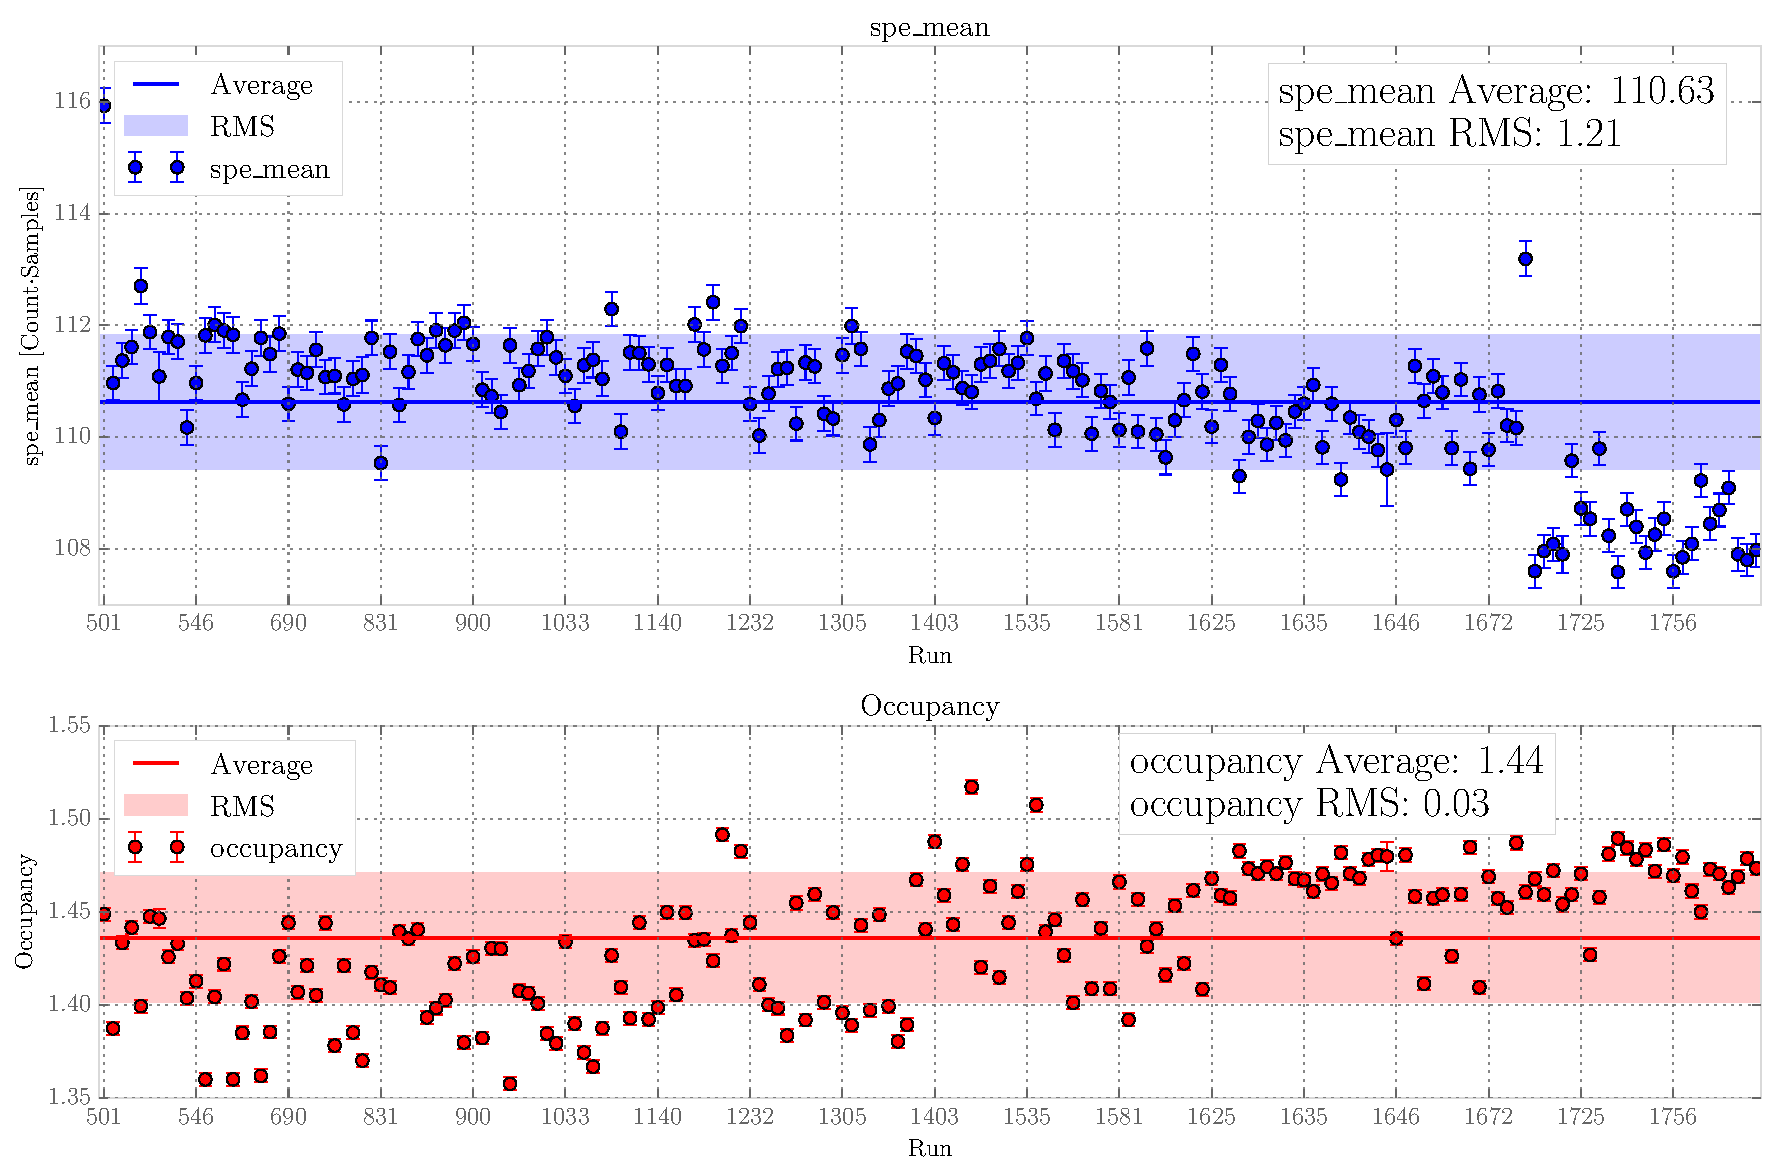
\includegraphics[width=1.1\textwidth]{calibtreeall.pdf}
	\end{center}
\end{frame}

\begin{frame}{spe\_mean and occupancy}

	\begin{tikzpicture}
		\hspace*{-0.3in}
	    \node[anchor=south west,inner sep=0] at (0,0) {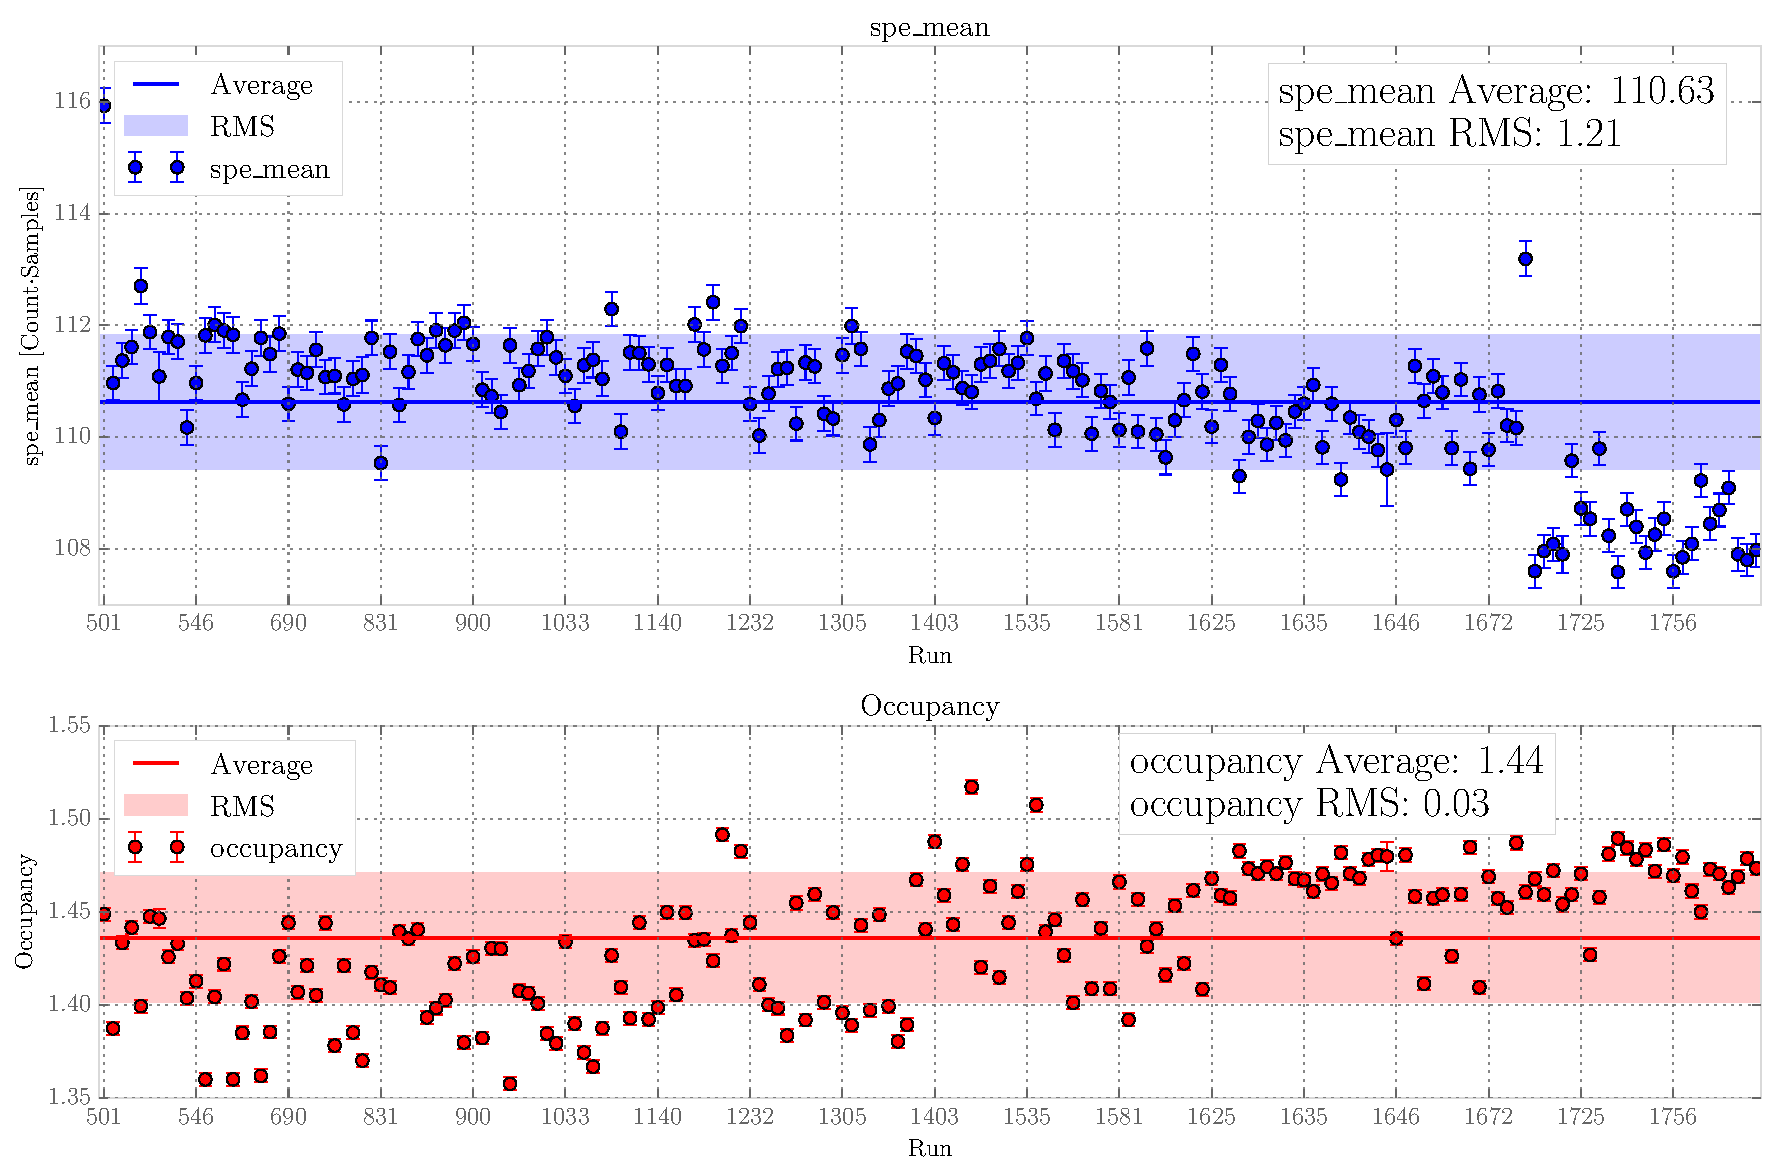
\includegraphics[width=1.1\textwidth]{calibtreeall.pdf}};
	    \draw[red,ultra thick,rounded corners] (9.5,6.4) rectangle (12.0,3.2);
	\end{tikzpicture}
\end{frame}

\begin{frame}{gauss\_center and spe\_sigma}
	\vspace{-1.1em}
	\begin{center}
	\hspace*{-0.3in}
		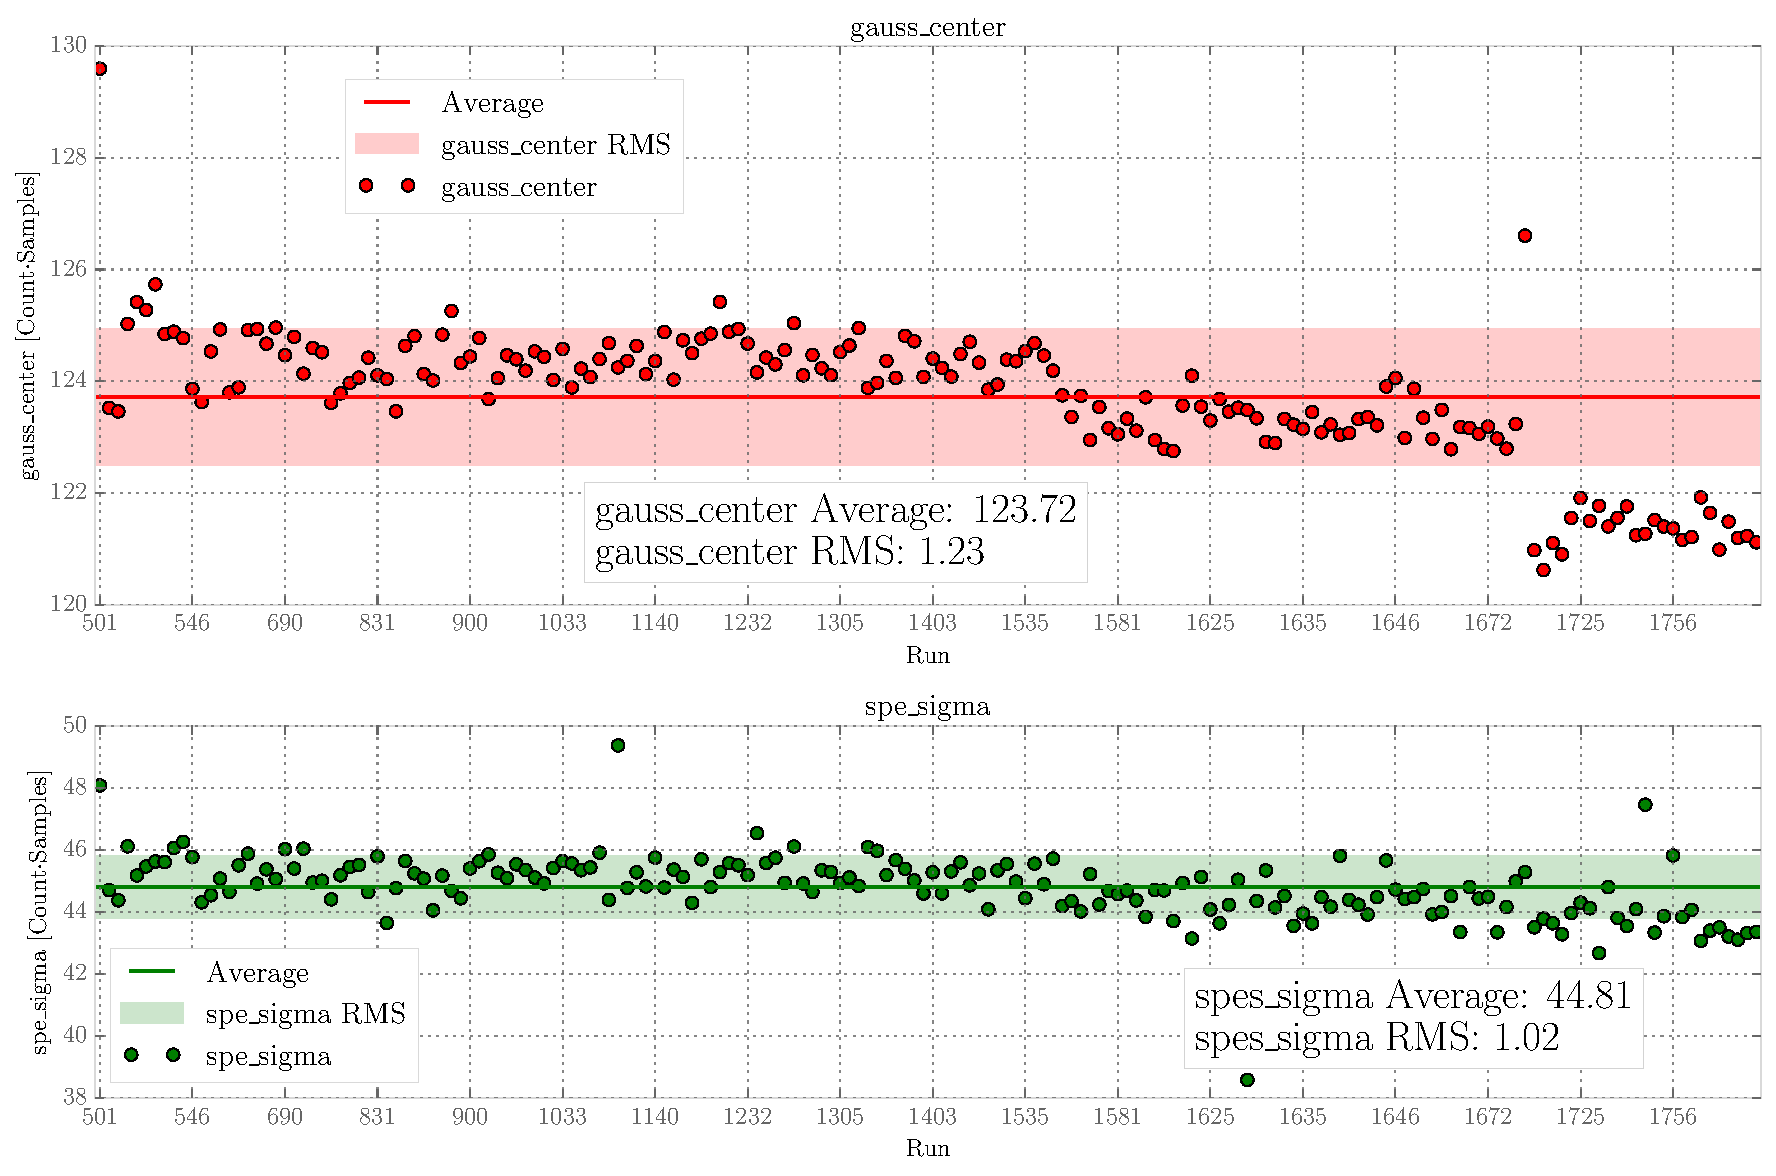
\includegraphics[width=1.1\textwidth]{calibtreeall2.pdf}
	\end{center}
\end{frame}

\begin{frame}{Further Steps}

	In addition to looking through the ELOG to determine the cause for the drop in SPE mean, the following runs were not included in this study:

	521
	523
	524
	525
	526
	527
	1207
	1233
	1281
	1282
	1283
	1329
	1606
	1608
	1647
	1648
	1793
	1798
	
	\vspace{0.5em}
	
	Common problems:
	
	\begin{itemize}
		\item Low mean
		\item High uncertainty
		\item ``inf" or ``NaN" values
	\end{itemize}
	
	\vspace{0.5em}
	
	Also looking at the same parameters for runs of different sources or drift fields may be enlightening.
	
\end{frame}

\end{document}